\documentclass{beamer}

\usepackage{tikz}
\usetikzlibrary{arrows,automata,positioning}
\newcommand{\transition}[3]{\ensuremath{#1 \overset{#2 }{\longrightarrow} #3}}

\tikzset {
	->,
	>=stealth',
	initial text=$ $
    every state/.style={minimum size=0pt}
}

\usetheme{default}

\title{Introduction to Finite Automata}
\author{Fabrizio D'Angelo, Michal Hecko}
\institute{RedHat}
\date{\today}

\begin{document}
    \begin{frame}
        \titlepage
    \end{frame}

    \begin{frame}[fragile]
        \frametitle{Example problem}
        
        \textbf{Task:} write a C function \texttt{is\_str\_rh(char* word)} that returns 
        \texttt{1} iff the given word is \textit{RedHat}.
        \pause  
        
\begin{verbatim}
int is_str_rh(char* word) {
    const char* rh = "RedHat";
    int i;
    for (i = 0; i < 6; i++) {
        if (word[i] == '\0')  break;    
        if (rh[i] != word[i]) break;    
    }
    return i == 6;
}
\end{verbatim}
    \pause
    
    What is the function state?
    \end{frame}

    \begin{frame}
        \begin{figure}
            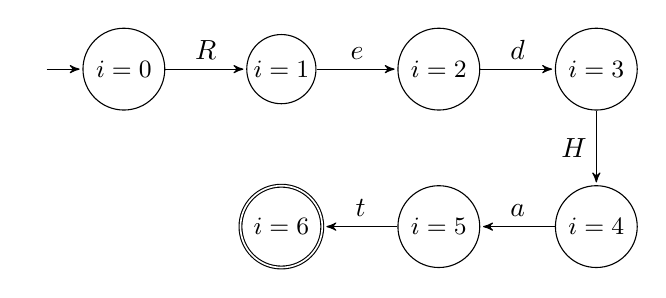
\begin{tikzpicture}[shorten >=1pt, node distance = 2cm, on grid, auto, initial text = $ $]
                \node[state, initial]                   (q_0)  {\small{$i = 0$}};
                \node[state, right of = q_0, inner sep=0]            (q_1)  {\small{$i = 1$}};
                \node[state, right of = q_1]            (q_2)  {\small{$i = 2$}};
                \node[state, right of = q_2]            (q_3)  {\small{$i = 3$}};
                \node[state, below of = q_3]            (q_4)  {\small{$i = 4$}};
                \node[state, left of = q_4]            (q_5)   {\small{$i = 5$}};
                \node[state, left of = q_5, accepting] (q_6)   {\small{$i = 6$}};
                
                \draw
                    (q_0) edge [above] node {$R$} (q_1)
                    (q_1) edge [above] node {$e$} (q_2)
                    (q_2) edge [above] node {$d$} (q_3)
                    (q_3) edge [left]  node {$H$} (q_4)
                    (q_4) edge [above] node {$a$} (q_5)
                    (q_5) edge [above] node {$t$} (q_6)
                    ;
            \end{tikzpicture}
            \caption{State space of \texttt{is\_str\_rh(char* word)}}
        \end{figure}
    \end{frame}

    \begin{frame}
        \frametitle{Formal definition of the model}
        Why?
        \begin{enumerate}
            \item study the entire class of similar problems mathematically
            \item decouple the problem structure from the implementation
        \end{enumerate}
    \end{frame}

    \begin{frame}
        \frametitle{Formal definition of the model}
        A \textit{finite automaton} $\mathcal{A}$ is the 5-tuple $(Q, \Sigma, \delta, Q_0, F)$, where:
        \begin{enumerate}
            \item $Q$ is a finite non-empty set of states,
            \item $\Sigma$ is a finite non-empty set of symbols called an~alphabet,
            \item $\delta \subseteq Q \times \Sigma \times Q$ is the set of transitions,
            \item $Q_0 \subseteq Q$ is the set of initial states, and 
            \item $F \subseteq Q$ is the set of final states.
        \end{enumerate}
    \end{frame}

    \begin{frame}
        \begin{figure}
            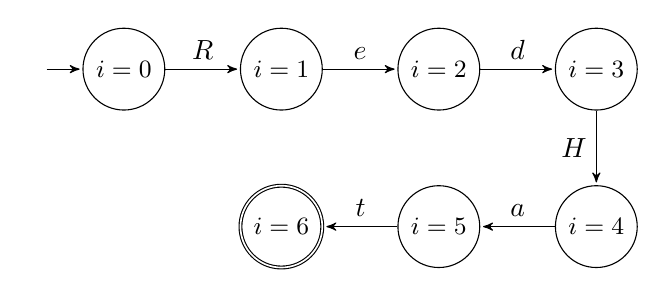
\begin{tikzpicture}[shorten >=1pt, node distance = 2cm, on grid, auto, initial text = $ $]
                \node[state, initial]                   (q_0)  {\small{$i = 0$}};
                \node[state, right of = q_0]            (q_1)  {\small{$i = 1$}};
                \node[state, right of = q_1]            (q_2)  {\small{$i = 2$}};
                \node[state, right of = q_2]            (q_3)  {\small{$i = 3$}};
                \node[state, below of = q_3]            (q_4)  {\small{$i = 4$}};
                \node[state, left of = q_4]            (q_5)   {\small{$i = 5$}};
                \node[state, left of = q_5, accepting] (q_6)   {\small{$i = 6$}};
                
                \draw
                    (q_0) edge [above] node {$R$} (q_1)
                    (q_1) edge [above] node {$e$} (q_2)
                    (q_2) edge [above] node {$d$} (q_3)
                    (q_3) edge [left]  node {$H$} (q_4)
                    (q_4) edge [above] node {$a$} (q_5)
                    (q_5) edge [above] node {$t$} (q_6)
                    ;
            \end{tikzpicture}
        \end{figure}

        In our example:
        \begin{enumerate}
            \item $Q = \{i=0, i=1, i=2, i=3, i=4, i=4, i=5\}$,
            \item $\Sigma = \{R,e,d,H,a,t\}$,
            \item \small{$\delta = \{\transition{(i=0)}{R}{(i=1)}, 
                              \transition{(i=1)}{e}{(i=2)},
                              \transition{(i=2)}{d}{(i=3)},
                              \transition{(i=3)}{H}{(i=4)},
                              \transition{(i=4)}{a}{(i=5)},
                              \transition{(i=5)}{t}{(i=6)}
                            \}$}
            \item $Q_0 = \{(i=0)\}$
            \item $F = \{(i=6)\}$
        \end{enumerate}
    \end{frame}

    \begin{frame}
        \frametitle{Richer automaton}
        \begin{figure}[h]
            \centering
            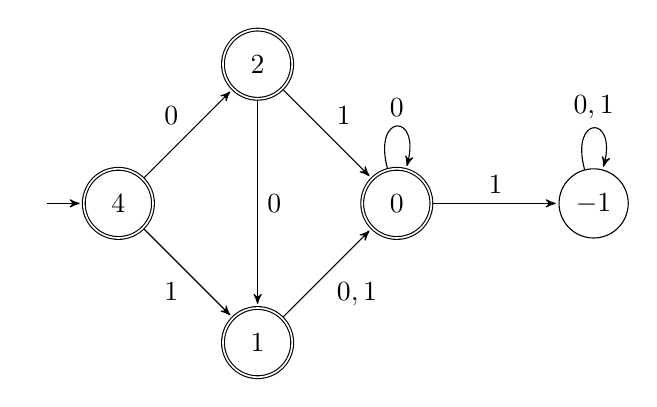
\begin{tikzpicture}[shorten >=1pt, node distance = 2.5cm, on grid, auto, initial text = $ $]
                \node[state, initial, accepting]               (q_4)  {$4$};
                \node[state, above right of = q_4, accepting]  (q_2)  {$2$};
                \node[state, below right of = q_4, accepting]  (q_1)  {$1$};
                \node[state, below right of = q_2, accepting]  (q_0)  {$0$};
                \node[state, right of = q_0]                   (q_m1) {$-1$};
                
                \draw 
                    (q_4) edge [above left] node {$0$} (q_2)
                    (q_4) edge [below left] node {$1$} (q_1)
                    (q_2) edge [right] node {$0$} (q_1)
                    (q_2) edge [above right] node {$1$} (q_0)
                    (q_1) edge [below right] node {$0, 1$} (q_0)
                    (q_0) edge [loop above] node {$0$} (q_0)
                    (q_0) edge [above] node {$1$} (q_m1)
                    (q_m1) edge [loop above] node {$0, 1$} (q_m1)
                    ;
            \end{tikzpicture}
            \caption{Automaton $A_{\varphi}$ for the inequality $\varphi \colon x \le 4$ over $\mathbb{N}$}
            \label{fig:automatonIneqToDFA}
        \end{figure}
    \end{frame}

    \begin{frame}
        \frametitle{Determinism}
        Notice our definition ($\delta \subseteq Q \times \Sigma \times Q$) allows nondeterminism: 

        \begin{figure}[h]
            \centering
            \begin{tikzpicture}[shorten >=1pt, node distance = 2.5cm, on grid, auto, initial text = $ $]
                \node[state, initial, accepting]    (q_0)  {$q_0$};
                \node[state, above right of = q_0]  (q_1)  {$q_1$};
                \node[state, below right of = q_0]  (q_2)  {$q_2$};
                
                \draw 
                    (q_0) edge [above left] node {$a$} (q_1)
                    (q_4) edge [below left] node {$a$} (q_2)
                    ;
            \end{tikzpicture}
        \end{figure}
        We say that automata that satisfy our original definition are nondeterministic finite automata (NFAs).
        
    \end{frame}

    \begin{frame}
        However, allowing deterministic automata have some interesting properties (e.g. easy interpretation).
        Therefore, we define a deterministic finite automaton (DFA) to be a FA $\mathcal{A}$ that further satisfies:
        \begin{itemize}
            \item $\delta$ is a function,
            \item $|Q_0| = 1$ (there is only one initial state).
        \end{itemize}.
    \end{frame}

    \begin{frame}
        \frametitle{Important definitions}
        \begin{itemize}
            \item A word $w$ is a sequence of alphabet letters ($w \in \Sigma^*$).
            \pause

            \item A \textbf{run} $r$ of a automaton $\mathcal{A} = (Q, \Sigma,
                \delta, Q_0, F)$ over a word $w$ of length $n$ is a sequence of
                states $r = q_0, q_1, \dots q_n$ ($q_i \in Q$ for $0 \le i < n$)
                such that $q_0 \in Q_0$, and for every $1 \le i \le n$ there is
                a transition $\transition{q_{i-1}}{w_i}{q_i}$.  \item A run is
                    \textbf{accepting} iff $q_n \in F$.  \pause

            \item A language of an automaton is a set of all words for which an accepting run of $\mathcal{A}$ exists.
        \end{itemize} 
    \end{frame}

    \begin{frame}
        \frametitle{Equivalency of DFAs and NFAs}
    \end{frame}

\end{document}
